\chapter{Conclusion: Where Next for Molecular Studies of CFTR}
\label{chap:conclusion}
\begin{chapquote} {Eduardo Perozo (personal communication)}
We have more problems than hands. 
\end{chapquote}


\section{Summary: The Three Categories for Future CFTR Studies}

The preceding chapters have fit into some broad themes. Chapters \ref{chap:introduction} and \ref{chap:methods} outlined a philosophy of biological physics which we seek to use to understand Cystic Fibrosis. Meanwhile chapters \ref{chap:I37R}-\ref{chap:opening} built up a molecular understanding of the root cause of Cystic Fibrosis and what a new class of drugs are doing to treat it. In this chapter we will tie these results together. We will build a physical perspective on the rescue of mutant CFTR by potentiator drugs. A similar model could be built for corrector drugs, or even used to think about the modulation of any protein by small molecules.


We will begin with a brief overview of our results so far, analysing 4 rare CF-causing mutations which appear to respond to CFTR modulators even though they each have a unique molecular defect. We will then look at the molecular details of one of the best studied and most common disease causing Mutations G551D. 

We will show through simple unbiased MD that this mutation causes a disruption to the binding of ATP, resulting in a gating defect. As with previous chapters, this gating defect appears unique, sharing little in common with the other gating defects we analysed previously. This array of different disease phenotypes leads us to propose a model based on the gating energy landscape, which accounts for the rescue of unique phenotypes by a class of drugs all acting with the same mechanism of action. 


%Our simulations of G551D and Q1291H appear to show a similar molecular phenotyope, even though they occur on different parts of the protein. Q1291H is an extremely rare mutation, it has not been clinicarlly characteriesd and is not approved for treatment with modulators. So, by studying a common mutation, G551D and comparing it to Q1291H we give an example of theratyping of CF mutations from the molecular level.

We will end this chapter by giving some directions and studies for the necessary work to complete this model. These directions will address 3 areas 

\begin{itemize}
	\item A basic understanding of the function of CFTR.
	\item Granular classification CF-causing mutations and the biophysical basis for their misfunction.
	\item Elucidating the molecular mechanism of action of different CFTR modulators. 
\end{itemize}

We will also suggest \textit{in silico} studies to further research in each of these areas.

The most important category not listed in the above, and sadly completely beyond the reach of our computational capabilities is is a molecular and cellular understanding behind the heterogeneous patient response to modulators, even between patients with the same defect. Identification of which genetic and cellular factors give rise to this phenomenon will be critical to the development of personal medicine in CF. \textit{Ab initio} studies of the folding energy of CFTR mutations would lead us to expect that the majority of missense mutations produce defects less deleterious than the more common $\Delta$F508. This means that with the optimal choice of modulators tailored to each patient, we can optimally rescue the CFTR proteins being expressed in their bodies. Understanding the molecular and cellular basis behind these choices will be critical to these choices.

The preceding chapters have given technical and molecular details about the cause of Cystic Fibrosis by rare genetic mutations, and further demonstrated that these mutations may be treated by existing small molecule drugs. The unique molecular fingerprint of each mutation indicates that in order to deliver better outcomes to patients a more personalised approach is necessary to the choice of medication. 

In order to tie these results together, in this chapter I will propose a conceptual framework which explains how these drugs are able to treat such diverse molecular phenotypes. This model would appear to suggest that patients with rare missense mutations would be more likely to respond to respond to CFTR modulators. The implications of this model are also likely to inform the design of future generations of CFTR modulators. 

The model we will propose raises the importance of some outstanding fundamental questions about CFTRs structure and function. Some of these questions simulations are uniquely placed to answer and we will outline some studies to address them. 

As such, the areas which deserve the most attention for molecular studies of CFTR are to address the controversies surrounding its structure and elucidate the action of drug binding. Together these will allow a clearer understanding of CFTRs function in health and misfunction in disease, enableing more targeted drug development. Current generation modulators have been identified using high throughput screening, the new generation of high computational power, artificial intelligence and structural data will allow a more targeted, perhaps even mutation specific approach to the design of new modulators.

\section{Outstanding Basic Questions of CFTR Function}
In chapter \ref{chap:I37R}, \ref{chap:R352Q}, \ref{chap:S945L} and \ref{chap:opening} we have analysed a disease causing mutation in detail in order to understand \textit{how} it caused CFTR to misfunction. What have found is a large diversity of molecular phenotypes which may cause disease. What is thus remarkable is that the \textit{in vitro} component of these papers all demonstrate that these mutations are responding to the same drugs, albeit with differing efficacies.


This model has important implications. We should be giving more patients modulators. Missense mutations likely represent a small perturbation to the folding and gating landscape of the WT channel and such . I assert that any heterogeneous response to modulators is not in fact to do with the mutation or the modulators them selves but likely involves other protein systems. Some of the uncertainty can be alleviated by the use of pre-clinical models which should be able to clear . Currently a range of missense mutations are recomended for treatment by trikafta but . Their current exclusion from accessing these therapies is errant. The above model suggests that when a patient carrying such a rare mutation does not respond to modulator therapy, it is unlikely that the lack of aresponse is due to the inability of these modulators to rescue the function of CFTR. From the perspective of protein physics, $\Delta$F508 is likely to perturb the protein much more than any missense mutation \cite{}. Rather, it is more likely that if a patient does not respond to modulators it is due to the broader heterogeneous response to modulators found in all patients. 


There is no reason to believe that even in patients who do not show benefit from modulator therapy that the drugs are for some reason not reaching the CFTR protein. In fact, they seem to metabolise the drugs at the same rate as patients who do. There are significant unresolved questions as to why these modulators are not providing the benefit they should be to patients. The success of preclinical models indicates that the problem is the cellular level and not at the level of organs or tissues. There is probably some genetic or cellular component that has not yet been identified which, once addressed, could bring the benefits of modulators to these patients.






The above model in figure \ref{drug_action_model} gives a rational, physical basis for the wide range of molecular phenotypes that CFTR modulators appear capable of treating. This same model would appear to argue that for most missense mutations we would expect them to respond to some sort of CFTR modulator. In short, the preceding chapters have shown that CFTR may misfunction by a wide range of defects. 

The ongoing discovery of rare mutations highlights the importance of this personalised approach to the treatment of CF. The process for developing potentiator class drugs was by studying the G551D mutation. Drugs that were found to restore function for this rare mutation are now widely used by sufferers of cystic fibrosis \cite{vangoor2009}. The study of rare mutations N1303K which currently do not respond to certain modulators may lead to the discovery of more effective compounds to treat cystic fibrosis such as. Thus, the approach to the treatment of Cystic Fibrosis is intersectional, as more rare mutations are discovered and treated the better the outcomes for all patients with Cystic Fibrosis will be. Each rare mutation sheds light on the function of CFTR and lets us understand and treat the root cause of the disease better.

One of the most important studies to understand the basic function of CFTR is the characterisation of its full gating cycle. This will aid in the generation of new potentiators, but also serve as an important mile-stone in computational biophysics. CFTR has been very well studied and os we understand the energetics and the kinetics of its gating very well \cite{csanady2017}. Matching these the predictions would demonstrate the , recent simulations of the covid spike protein have demonstrated this is likely possible with current forcefields \cite{casalino2021}. Cryo-EM structures of ABC transporters in transient states could be used to seed a SMwST or an eBDims calculation \cite{hofmann2019, orellana2016, roux2021, pan2008}. We have both the open and closed states of the human channel, a tragetted MD methodlogy coudl link them together \cite{zhang2018, liu2017, moradi2015}.

\subsection{Addressing Controversies Surrounding the Structure of CFTR}

Since the release of full length CFTR structures there have been some controversies surrounding their structure. These centered around the unusual conformation of TM8.

There are sadly few examples where membrane proteins have been characterised in both in both detergents and detergent micelles and nano discs revealed different side-chain conformations (however, the backbone was conserved) \cite{autzen2019, gao2016, cheng2015}. 


%\begin{figure}
%	\label{ABC_diversity}
%	\begin{center}
%	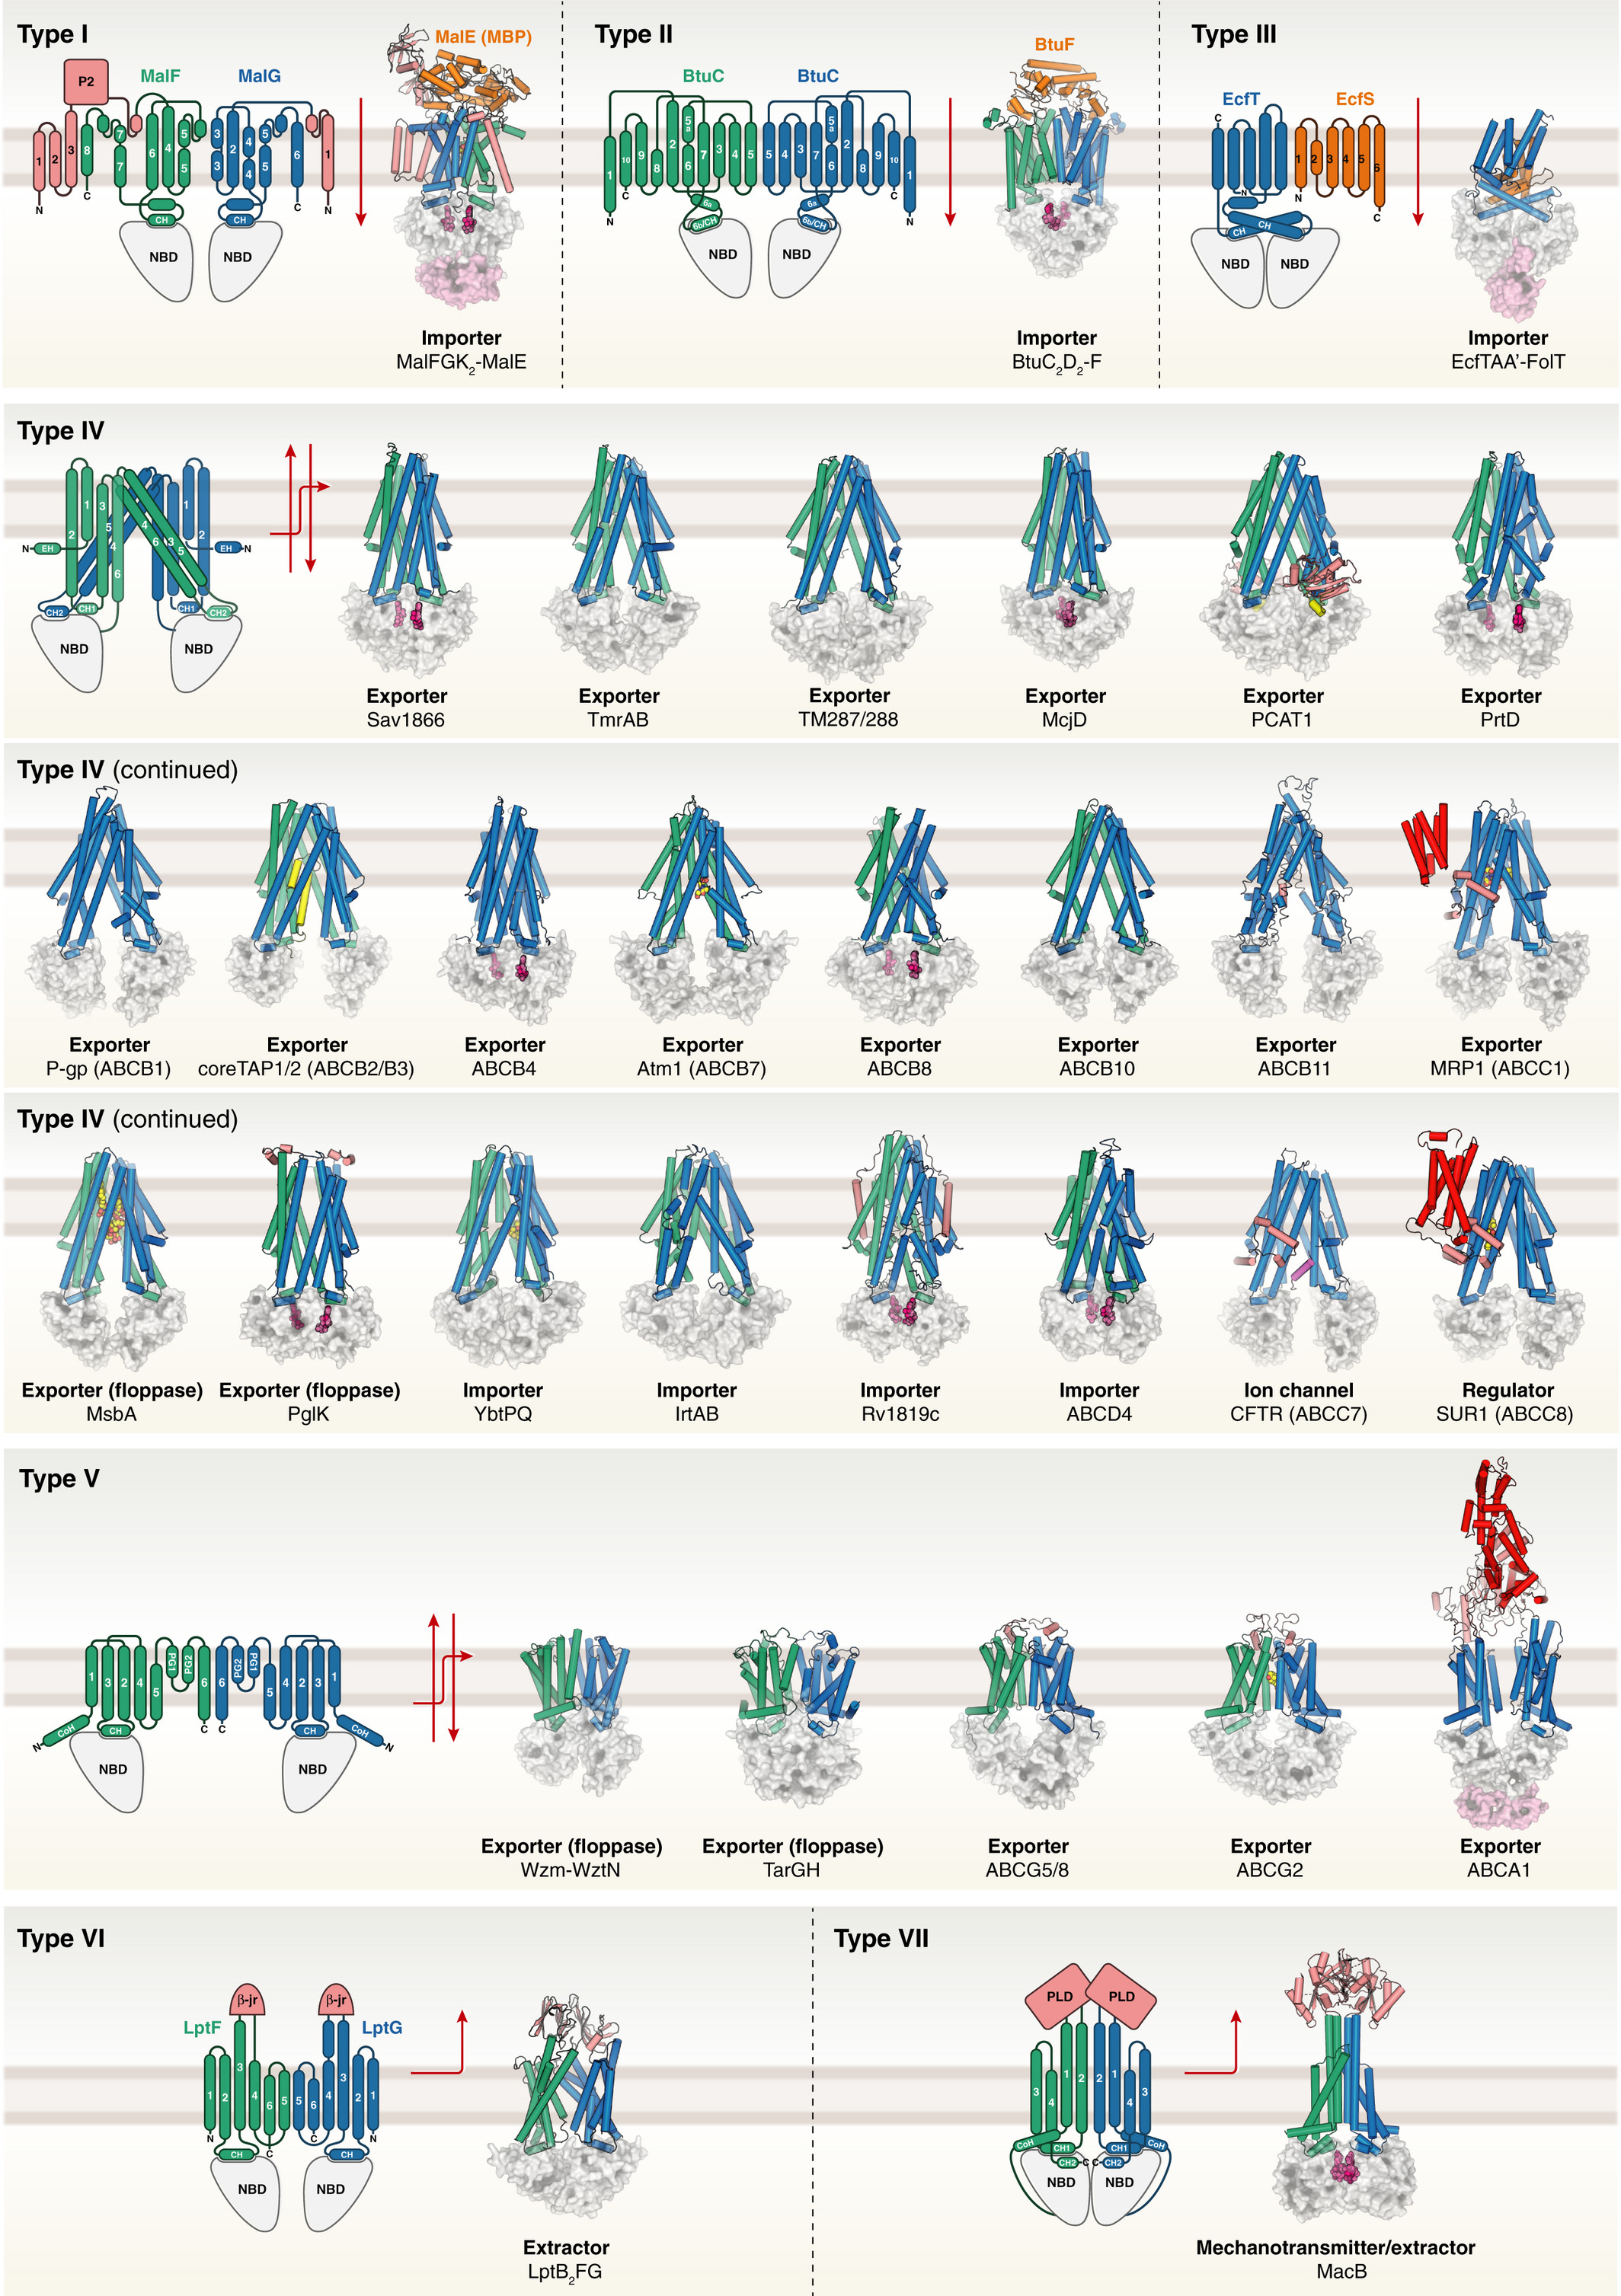
\includegraphics[width=\textwidth]{figures/ABC_classification.jpg}
%	\end{center}
%	\captionsetup{singlelinecheck = false, justification=raggedright}
%	\caption[CFTR Structure] {\textbf{CFTR Structure}}{The structural diversity of ABC transporters. Structures are classified based on the organisation of their TMDs source \cite{thomas2020}.} 
%\end{figure}

ATP-Binding Cassette (ABC) transporters are an intriguing super family of proteins. On the whole, they transport substrates by using the energy from ATP hydrolysis. These can be diverse substrates such as lipids or small molecules. Their structural diversity can be seen in figure \ref{ABC_diversity} reflecting their array of functions. 

CFTR is unique, as it is not a transporter, but rather an anion \textit{channel}. The kinetic energy of the ATP is not used to translocate substrate across the membrane but rather simply used in the regulation of the gating cycle. There is ongoing debate about how closely hydrolysis is coupled to the diffusion of ions \cite{}. Chloride, bicarbonate and other anions are able to passively diffuse through the channel. This evolutionary misappropriation of a transporter to a ``leaky channel" is perhaps the reason so many mutations can create a non-functional protein \cite{depristo2005,linsdell2018}.

CFTR belongs to a super family of proteins known as ATP Binding Cassette Transporters,  many of these proteins perform active transport across cell membranes. The substrates they transport can vary, including lipids and drug molecules. Proteins in this family share a common motif known as Nucleotide Binding Domains (NBDs). These domains act as ATPases, accelerating the hydrolysis of ATP. The energy from hydrolysis is then transferred into the protein in order for it to pump its substrate against a concentration gradient. 
The most recent structure of human CFTR in a phosphorylated environment has some interesting features which have lead to some controversies in the literature. After spending significant time researching them I have conducted an extensive literature review in order to learn more about of these concerns. The released structure of activated, human CFTR has two features that have caused some in the CF field to suggest issues with this structure. Firstly, this structure is not sufficiently open to conduct chloride ions. Chloride ions have a diameter of 1.7$\angs$ while the structure has a constriction of 1.1$\angs$\cite{zhang2018}. So, there must be some level of conformational changes, even if chloride were to move through the channel completely dehydrated. This becomes even more of an issue when considers the experimental evidence where much larger anionic species such as bicarbonate and glutathione were shown to permeate through the channel \cite{kogan2003}. This suggests that there is a much larger conformation which has not been observed experimentally or in simulations. This was the motivation for chapter \ref{chap:opening} of this thesis. Some studies have been performed in order to study the possible permeation paths of chloride but they were usually not carried out on hCFTR or have not addressed the pressing question of how larger ions might permeate the channel \cite{farkas2020, zeng2021}. Bicarbonate in particular is of great physiological importance as there is a high correlation between the channel's ability to permeate bicarbonate and the pancreatic sufficiency of a patient carrying the mutation \cite{}. In light of this, structural knowledge of a fully open conformation of CFTR is critical to a personalised approach to the treatment of CFTR.

The second and harder to resolve controversy concern the role of TM8. This transmembrane helix has an unusual bend in the middle of the plasma membrane. This is not something seen before in ABC transporters of this type. So it has led to some open questions as to how this bend might contribute to the function of the channel \textit{or} how it might be an artifact of the imaging process. For the former case, the structural biologists in the Chen lab proposed a mechanism whereby the upper hinge of TM8 swings 55$^o$ during the transition to the open state. This mechanism would give justification of the pathogenesis of certain mutaions such as L927P. 

The arguments for the bend in the helix appear to be unphysical. In cryoEM structures, we can observe that the bent conformation is stabilised by salt bridges R347-D924 and E873-R933. The former bond has been well studied experimentally and was expected in the 3d structure. Additionally, all hydrogen bonds along the in the bent helix are . Been observed to be stable in MD \cite{corradi2018} .  is energetically stable.

Finally, simulations of both human and zebra fish structures were used to study the stability of TM8 \cite{corradi2018}. As we will discuss in detail in chapter \ref{chap:perspective} all CFTR structures solved by the Chen lab exhibit an unusual fold in TM8 \cite{fiedorczuk2021, liu2017, liu2019, zhang2016, zhang2018a, zhang2017a}. The helix unwinds in the middle of the membrane, a configuration that was initially thought to be energetically unfavourable but more recent studies have supported this conclusion. This prompted some questions surrounding the protocols used to purify and image the protein. Hence, simulations were employed in order to test whether this kinked configuration would be stable in a lipid bilayer surrounded by a solvent. It was found that the kinked configuration of TM8 was indeed stable on microsecond timescales, with some interesting deformations introduced to the surrounding membrane \cite{corradi2018}. The simulations of hCFTR in this thesis have also been consistent with these findings. These results indicate that this unusual conformation of TM8 is likely correct. Additionally, \textit{in vitro} findings would also appear consistent with this conformation of TM8 \cite{infield2021}. In particular, it was demonstrated that disulfide bridges could be  spontaneously formed when cysteines were substituted in place of Y914 on TM8 and L102 on TM1, as well as other pairs of amino acids on both TM8 and TM6 \cite{negoda2019}. This stood as strong evidence that TM8 is a pore lining helix, consistent with the kinked conformation observed in cryo-EM studies.

However, there are still some unanswered questions for the discrepancy between the solved human and solved chicken structures. Certain salt bridges are not present in the latter structure and so single channel electrophysiology experiments may be able to resolve these issues. For example, in 6MSM, the human structure of CFTR there is a salt bridge between amino acids 933 and D873 which is not present in the chCFTR structures. This bond is also present in the zCFTR structure 5W81. If a charge swapped mutant such as R933E/E873R restores WT-like gating behaviour to the channel it would be  strong evidence for the unwound conformation of TM8. 

The two proposed conformations also have vastly different ion permeation pathways, and so blockers engineered to target one conformatoin over the other would also go a long way to answering these questions. The available evidence strongly favors the R334 pathway between TM1 and TM6. Such as experiments to  demonstrate the blockage of current with zinc have shown that mutations to R334 strongly suggest that chloride permeates along this route. Additionally, trhere are several disease causing mutations in the region surrounding R334, such as R334W, R117H, E116K, D110H, I336K \cite{cftr2}. This permeation route also explains the rationale behind the gain of function mutation F337A \cite{}. Determining which model is correct has wide implications for creating the next generation of mutation targeted potentiator class drugs.

\cite{gao2015} also concluded that the chloride opening lined TM6. The findings that TM1 and TM6 move apart form eachother in \cite{negoda2018} also support this conclusion (this is also more consistent with our open model in chapter \ref{chap:opening}). Which is more consistent with the 6MSM model than the chicken structure.
The chicken structure has undermised NBDs, this is inconsistent with biochemical assays that dimerisation is tightly coupled to the dimerisation of NBDs \cite{vergani2005, yeh2021}.

Mutagenesis studies of the outer pore would strongly support the Chen structure over the chicken streucture. In particular, Paul Linsdell performed very careful experiments to measure blockage chloride blockage and found that several residues play an important role in the permeation of chloride in the outer pore. In the chicken structure these residues are occluded and far from the chloride permeation pathway. However, in the Chen structure they appear to play an important role in the permeation of chloride. This will be discussed in detail in \ref{chap:opening}.

A study assessing the accuracy of Alphafold's predictions of transmembrane protein structures found an intersting result. When alphafold made predictions that involved the use of templates it predicts the unwound conformation of TM8. On the other hand, when templates are removed from alphafolds predictions it predicts a straight TM8 conformation, very similar to that found in chCFTR. The authors of this study suggested the reason for the discrepancy was due to the use of detergents in the deteremination of the structure of hCFTR. However, careful reading of cryo-EM literature reveals no examples where the use of detergents has resulted in such drastic conformational changes. One of the few examples where both detergents and native-like nanodisks were used to determine the structure of a protein are the determinations of the structure of TRPV1. These studies revealed no difference to the backbone helices but did suggest important information about the importance of different interactions with lipids \cite{gao2016}. A lot of work has been performed in order to create detergents which reflect a native lipid environment and these are the species that were used in the determination of the human CFTR structure (albeit at a higher than optimal concentration) \cite{gao2016, zhang2018, kampjut2021}. 

%The authors of the chCFTR paper suggested that the different expression systems used in the two studies could be the reason for the discrepancy between the two systems, due it their different post translational processing apparatus. Although both groups used mammalian cell lines the chCFTR paper used hamster? cells \cite{aleksandrov2015} and the Chen lab used HEK293S cells. The chicken structure also underwent significant mutations in order to be locked open and imaged. The regulatory insertion was deleted in order to aid in the purification of the protein. 

Figure \ref{} shows the large diversity of structures in type IV ABC transporters, many of which also exhibit bends within transmembrane helices \cite{thomas2020}. Although none of these structures exhibit such a bend in TM8 specifically, the 

\cite{negoda2019} gives strong evidence that TM8 must line the conduction pore. Due to its proximity to F337 and other pore lining amino acids. This is more consistent with the Chen structure than the chicken structure where 337 is far from the conduction pore. Their findings are also consistent with our open structure, proposed in \ref{chap:opening}, where distances between the cross linked sidechains F337C/Y914C, are found to be very stable in experiment, but the sidechains of L102C/Y914C are found to be more exposed to the extracellular environment. In the chicken structure no such cystine crosslinking would be possible as TM8 is too far from TM1 and 6 for these sidechains to link. This is strong evidence for the Chen structure.

These controversies have recently been resolved by careful work from the laboratory of Jonathan F. Fay to reconstitute and image CFTR in a nanodisc \cite{aleksandrov2022}. This technique seeks to understand membrane proteins in a physical environment which more closely reflects what is find \textit{in vivo} \cite{}. In this study, the authors found that TM8 exhibits signicant flexbility, favoring the kinked conformation found by the Chen lab.

Ultimately, this is a difficult problem in all structural biology. Even though we are gaining an unprecedented view into protein physics with the resolution revolution we have still only sampled an extremely small part of sequence space. With all our cryo-EM, simulations and biochemical assays we still have much to learn about these incredible molecular machines.



This model makes clear what the pressing questions are in molecular cystic fibrosis research. Firstly and fundamentally, there is the task of finding the molecular details of the energy landscape in figure \ref{drug_action_figure}.  This would likely be the most computationally and theoretically demanding step in the proposed pipeline. However, it could be accomplished with limited input from experimental and clinical sources. Since we have the inactive, active and confomrations of CFTR, the minimum energy pathway between them could be calculated using path-CV or SMwST methods. This is likely within reach of current computational capabilities but would be very involved. A related project would be to perform such a calculation on an ABC transporter with more structural information, to validate the methodology. This first step forms the basis of the rest of the proposed model. The two preceeding steps rely on calculating changes to it based on the introduction of drugs or mutations.

The second part of this program, will be to elucidate where and how mutations modify this energy landscape, to produce a folding or a gating defect. Each mutaiton will have a specific fingerprint, it will produce barriers and valleys in this landscape in specific places and specific heights. As we have seen, G551D . We expect that a seemingly unrelated mutation Q1291H will produce a similar barrier to the gating transition. This leads us to expect that these two mutations will both respond to the same kinds of modulators. This step will require some input from clinicaans and epxerimetnal laboratories in order to investigate hte cellular phenotype of each mutation. This will aid in the categorisation efforts, considering that there are orthogonal derees of freedom that are simply too slow to sample in MD.

The final element in this program is to understand, mechanistically, how small molecule drugs are compensating for the modified landscape exhibted by mutations. There are several unanswered questions surrounding how modulators restore CFTR function, but these are being studied intensly \cite{}. We propose that in silico characterisation, in parralel with these in vitro effors twill aid in efforts of both theratyping and drug discovery. As was observed in \ref{chap:cftr} the close integration of simulation studies ameliorates some of the challenges inherent to a computational appraoch. Therefore, we propose that future in silico efforts to elucidate the drug binding pockets of CFTR remain tightly integrated with in vitro experiments, until ocmputational methods are more mature. However, for already proposed drug binding pockets such as those proposed in \cite{}, it is likely that alchemical free energy calculations could provide significant mechanistic insight into he function of these CFTR modulators. These studies should be a priority for molecular studies of CFTR as they will have significant implications for drug discovery efforts and \textit{in vitro} investigations of these mechanisms can be challenging due to the hydrophobic nature of these drugs \cite{csanady2019}. 


Given that $\Delta$F508 may be rescued by triple therapy, we would expect the vast majority of missense mutations to also be amenable to pharmacological rescue. The $\Delta$F508 mutation in fact represents a far more deleterious effect on CFTR the protein than many missense mutations, \cite{bahia2021}. Hence, from a biophysical point of view, it makes little sense to exclude patients carrying missense mutations from access to modulator therapy. The rational for such exclusion is based upon the extreme cost of the drugs alongside the unpredictability of patient response. However, in these patients carrying this rare mutations, the heterogeneity of their response to these medications is not likely to be due to the interaction between the drugs and mutant CFTR. Rather, the failure of these patients to respond to these therapies is likely due to poorly understood molecular or cellular factors. Given the findings of this study and others we encourage a more rational approach to hte inclusion patients missnese mutations in access to CFTR modulators \cite{}. 

The molecular and cellular basis behind this heterogeneous response is thus of critical importance to CF care and is only recently being addressed in the literature \cite{}. The metabolism of these drugs is under study, in order to understand this patient specific response \cite{hanafin2021}. A complimetnary therapeutic which addresses the root cause of this issue would greatly increase patient outcomes. Sadly, such studies are far outside the reach of computaitonal biology at the moment and so we encourage careful clinical research to test for genetic or environmental factors which cause patients to not respond to modulators. In the mean-time, a pre-clinical approach such as the one undertaken by the collaborators of this thesis can rationally expand the number of patients who will receive these therapies.

Trikafta triple therapy is changing the face of mutation specific therapy. For example, N1303K, a common mutation, which does not respond to potentiators or correctors by thesemselves, or even together \cite{} does respond to triple therapy. This is a similar situation for rarer mutations like R560S, which is rarer and so has not yet been tested for efficacy with the triple therapy \cite{awatade2019}. In summary, given the results from this thesis we expect that the majority of missense mutations will respond to a triple therapy. Patients carrying these genotypes who do not respond to triple therapy likely have factors \textit{beyond} the physical action of the modulators on CFTR which are . It is possible that exceptions do exist and the physical model proposed in this chapter will help us form a physical basis for which ones can be excluded. To account for these factors a patient specific pre-clinical approach will help us predict which patients respond to these medications and eventually pin down which cellular factors are preventing the rescue of chloride transport in these patients. The maturation of this technology will bring considerable therapeutic benefit to CF patients and eventually those suffering from other diseases too.

The limited success of this work demonstrates the increased understanding molecular medicine can bring to patients. Should the above model prove successful, such an approach approach to personalised medicine could  be considered when studying other monogenic diseases such as Muscular Dystrophy, Sickle Cell Anemia and Huntington's disease \cite{}.  Once single genes are understood the understanding could be built outward to encompass more complex diseases which involve the interactions between many genes such as diabetes and cancer. 

An analogous model could be drawn for the action of correctors. To do this we would need to clearly delineate the folding pathway of the CFTR protein and study how mutations cause aberrations in the folding landscape. Although work on this has begun \cite{krainer2018, kleizen2021, kleizen2020, fiedorczuk2022}, the folding pathway is much less straight forward to simulate than the gating pathway. Since we can clearly delineate the different events in the energy landscape of CFTR gating, like ATP binding and pore formation, we will build our model with a focus on this aspect of protein function. Nonetheless, the concepts are transferable, to CFTR folding and as more corrector class drugs are developed and more mutant forms of CFTR are imaged we will gain more understanding f the folding pathway of this critical protein, so in time this model can be transferred to correctors as well. Additionally, as computer models improve we can simulate parts of this pathway as well. Computational capabilities are likely sufficiently advanced to simulate the full gating cycle of CFTR and so discover which parts of the landscape in figure \ref{drug_action_figure} are perturbed by mutations \cite{}. 

%These drugs are clinically efficacious \cite{VanGoor2014} on several mutants with some curious exceptions like N1303K. I suggest the following mechanism for their action. I suspect a similar analogy exists for the action of the correctors. WT-CFTR exhibits a natural landscape with kinetic barriers in the transition between the closed and open states. A gating class mutation to CFTR will introduce a kinetic barrier in the pathway of this conformational transition. What these drugs do is reduce a barrier in the existing conformational landscape of CFTR. This compensates for the barriers introduced by the mutation. j



The program outlined above allows us to direct other research efforts into the study of CFTR and the molecular nature of CF. 

Firstly, there are controversies surrounding the structure of this protein. Primarily determining resolving the physiologically relevant conformations of TM8 and the conduction pathway of ions through CFTR. Since the release of atomistic structures of CFTR, there .

Secondly, there are questions about how tightly the coupling of hydrolysis of ATP in the NBDs is to the conduction of ions.

\section{Mechanistic Understanding of Mutations}
As outlined in figure \ref{mutation_classes_figure} earlier, the molecular fingerprint of a mutation can be quite complex and ongoing work is needed to meaningfully group these mutations into more clinically meaningful categories. My prediction is that the conventional 6 classes will be more and more finely defined in order to choose CFTR modulators which are more specific to a patient's genotype and epithelial phenotype. 

Careful in silico in vitro and clinical experiments will be needed to adequately expand these 6 classes to more meaningful theratype.

In recent years there have been a slew of rare CF-causing genotypes discovered in populations with low rates of Cystic Fibrosis compared to Caucasians. These genotypes from Asia and the Middle East are often ultra-rare leading to poor outcomes for these patients \cite{}. 

\section{Elucidating Modulator Action on CFTR}
Closely related to the above two categories is the mechanism of action for existing drugs and the development of new drugs. The reason we were able to discover potentiator class drugs is through the study of a rare mutation. High throughput screening of small molecules in restoring the gating class mutation G551D led to the discovery of gating class drugs. In this way we can see how the study of rare CF can lead to better outcomes for all sufferers of the disease. This is especially pertinent as more rare genotypes are discovered in non-Caucasian populations such as in Asia and the Middle East.  

Protocols have recently been developed to test \textit{where} on the CFTR protein drugs bind, which heralds exciting times for drug development \cite{laselva2022}. In silico experiments could compliment these new probes well \cite{}.

At the time of writing there are 3 studies which purport to have found binding sites for potentiator class drugs \cite{}. There appears to be a \textit {in vitro} consensus site near the TM8 helix bend, confirmed by mass spectrometry, mutagenesis studies and cryo-EM visualisation. However, \textit{in silico} confirmation of this site has remained difficult, possibly due to the presence of the lipid bilayer slowing kinetic investigations of this region. Enhanced sampling methods and alchemical methods would be well placed to investigate the biophysics of drug action at each proposed site. The careful, detailed kinetic investigations in \cite{csanady2019} also give important clues as to how we should expect drug action to work. Careful, structure led experiments have the potential to aid in the development of new potentiator class drugs. This is of critical importance to CF care. Currently, only Ivacaftor (VX-770)  is the only potentiator accessible to patients, and certain mutations respond poorly to this potentiator \cite{phuan2018, vangoor2014}. 

Additionally, it should be obvious from this work that the action of these drugs is are highly dependent on the molecular function of CFTR. These small molecule drugs \textit{select} for a physiologically present conformation, so we would wish to design molecules which select for conformations which deliver the most clinic benefit. This is non-trivial and I believe  combination of careful molecular experiments, such as those of from the laboratories of Tzyh-Chang Hwang,  Christine E. Bear, L\'aszl\'o Csan\'ady and Paul Linsdell \cite{linsdell2018, csanady2019, zhang2017b}, and molecular simulations such as those found in this thesis and studies from the labs of John Paul Monron and Isabelle Callebaut \cite{hoffmann2018}.

Although at the core of CF pathogenesis, the function and misfunction of CFTR is only one aspect of this systematic disease. Increasing consideration should be given to a quantitative approach to mesoscopic modelling at the level of tissues and organ systems \cite{volt2014}.

In summary, the important findings from these 4 modelling studies demonstrate that many people with CF are likely to respond to modulator therapy, even though they excluded from these treatments by regulatory agencies. A biophysical methodology when considering the action of CFTR modulators leads us to expect that most patients carrying missense mutations will respond to modulator therapy.

By combining this molecular understanding with \textit{ex vivo} pre-clinical models it appears as as though CFTR modulators are capable of treating a diverse set of unique molecular defects. If the recommendations of this thesis are taken on board, eventually computational and molecular understanding of CFTR will sufficiently improved to make predictions about the response of specific mutations to modulators.  

Currently, computational methods are not sufficiently developed in power or accuracy to theratype a mutation ab initio. Hence, we must rely heavily on the measurements of a patients' cells made \textit{in vitro}. However, as a more complete understanding of CF pathogenesis and patient genetics is built, we will be able to offload more and more of this clinical work onto computers.

As figure \ref{CF_life_expectancy} demonstrated back in chapter \ref{chap:cftr}, basic science discoveries concerning CF have had a direct effect on the life expectancy of patients. The work in this thesis is a small example of how abstract physical models, such as those outlined in \ref{chap:methods}, can be applied to help real patients in a community such as allowing patients in Sydney Children's hospital to access medications which could add decades to their life span. We are entering an exciting era of biophysical research where advances in theoretical methods, computing power and experimental techniques are beginning to drive advances in each other at a frenetic pace. An example can be seen in the development of Alphafold2. The maturation of cryoEM allowed the discovery of new protein folds which Alphafold2's machine learning algorithms could then learn from. Now that the algorithm had these folds in hand it could predict entire proteomes. This now means that structural biologists can use the predictions of alphafold to solve even more structures more quickly. Eventually, more and more of the experimental work currently involved in biology will move onto the silicon chip, while experimental techniques will advance in other areas. Similarly, the theoretical model argued for in this thesis will eventually allow for patient assessments to be made \textit{in silico}
